%% %%%%%%%%%%%%%%%%%%%%%%%%%%%%%%%%%%%%%%%%% %%
%% Elementos Pré Textuais
%% ----------------------
%% 
%% Segundo o manual do IFPI, eles devem ser os seguintes (nessa ordem):
%%  1. Capa (obrigatório)
%%  2. Folha de rosto (obrigatório)
%%  3. Errata (opcional)
%%  4. Folha de aprovação (obrigatório)
%%  5. Dedicatória (opcional)
%%  6. Agradecimentos (opcional)
%%  7. Epígrafe (opcional)
%%  8. Resumo (obrigatório)
%%  9. Abstract/Resumo em outra língua (obrigatório)
%% 10. Lista de Ilustrações (opcional)
%% 11. Lista de Tabelas (opcional)
%% 12. Lista de Abreviaturas e Siglas (opcional)
%% 13. Lista de Símbolos (opcional)
%% 14. Sumário (obrigatório)
%% %%%%%%%%%%%%%%%%%%%%%%%%%%%%%%%%%%%%%%%%% %%

%% 01: Capa
\imprimircapa



%% 02: Folha de Rosto
%% OBS: O asterisco indica que haverá ficha bibliográfica (só funciona para impressão frente-e-verso)
\imprimirfolhaderosto*



%% Ficha Catalográfica (acho que é melhor adicionar via \includepdf depois)
%% Se for incluir um outro PDF neste documento: 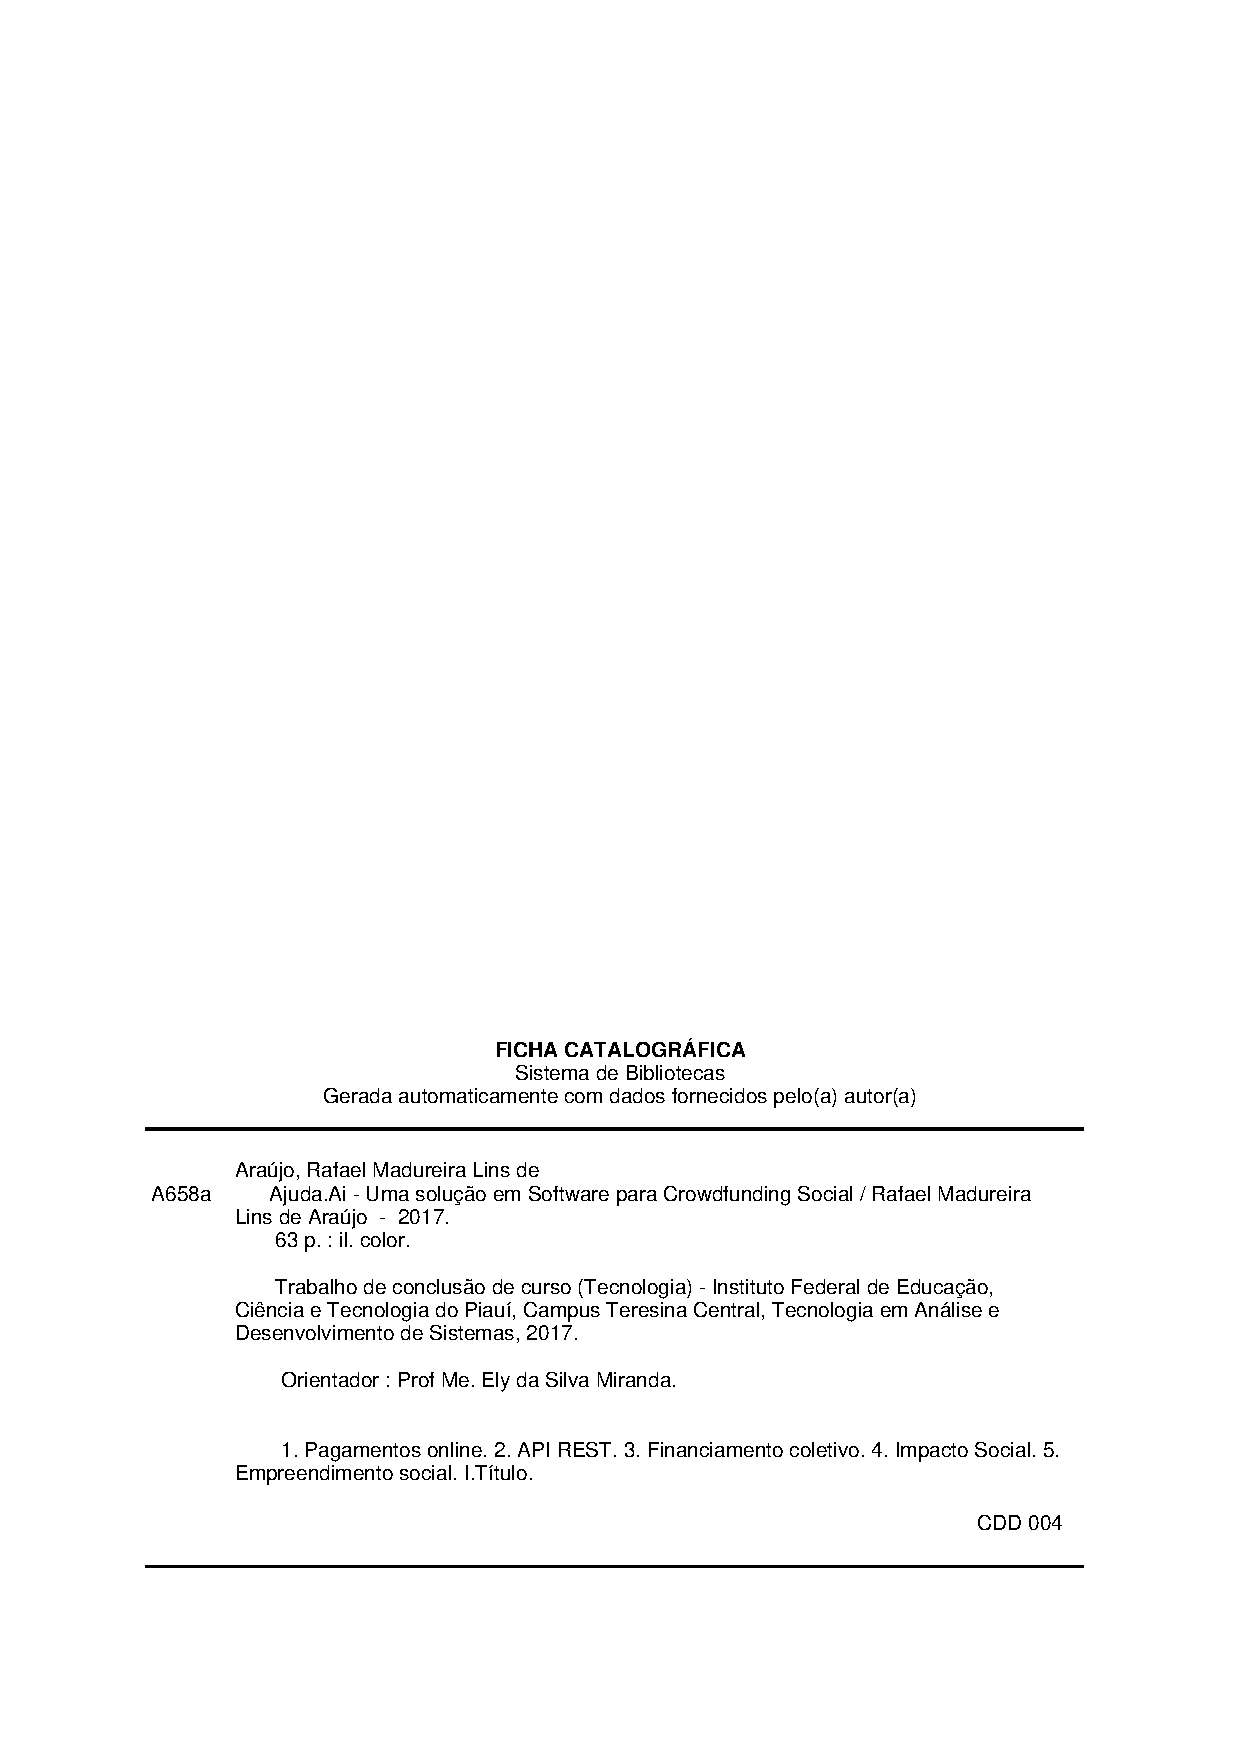
\includepdf{pasta-onde-está-a-ficha/ficha-catalografica.pdf}


%% 03: Errata
%% Errata
%\begin{errata}
%Elemento opcional da norma ABNT NBR14724 de 2011. Exemplo:
%
%\vspace{\onelineskip}
%
%FERRIGNO, C. R. A. \textbf{Tratamento de neoplasias ósseas apendiculares com reimplantação de enxerto ósseo autólogo autoclavado associado ao plasma rico em plaquetas}: estudo crítico na cirurgia de preservação de membro em cães. 2011. 128 f. Tese (Livre-Docência) - Faculdade de Medicina Veterinária e Zootecnia, Universidade de São Paulo, São Paulo, 2011.

%% Tabela de exemplo com os erros
%\begin{table}[htb]
%\center
%\footnotesize
%\begin{tabular}{|p{1.4cm}|p{1cm}|p{3cm}|p{3cm}|}
%  \hline
%   \textbf{Folha} & \textbf{Linha}  & \textbf{Onde se lê}  & \textbf{Leia-se}  \\
%    \hline
%    1 & 10 & auto-conclavo & autoconclavo\\
%   \hline
%\end{tabular}
%\end{table}
%
%\end{errata}



%% 04: Folha de Aprovação
\imprimirfolhadeaprovacao
%% Use esta se forem 4 membros na banca:
%\imprimirfolhadeaprovacaoduascolunas



%% 05: Dedicatória
%% Dedicatória do seu trabalho
\begin{dedicatoria}
	%% Empura o texto a seguir para a parte de baixo da página
	\vspace*{\fill}
    
    %% Alinhado a Direita
    \center
    \begin{flushright}
    	Dedico este trabalho a todos que acreditaram que ele sairia.
    \end{flushright}
    
    %% Descomente a linha seguir para deixar o texto centralizado verticalmente na página
    %% Lembre de comentar o "\begin{}" e "\end{}" acima para centralizar o texto da dedicatória.
	%\vspace*{\fill}
\end{dedicatoria}



%% 06: Agradecimentos
%% Agradecimentos
\begin{agradecimentos}
	Agradeço primeiramente a meus pais, família e Alaydes Morais que, assim como muitos, aguardaram pacientes pela conclusão do curso e me deram o apoio necessário para terminar a jornada.
    
    Agradeço aos amigos, virtuais e reais, pelas risadas, apoio, dicas e vários ``eu fiz meu TCC em \(N\) dias'' --- Em especial Rafael Soares, Rafarpo, Ebbitt, Rosenrot, Zenlee, Tajaro e Velinde.
    
    Agradeço profundamente aos mestres e professores que partilharam de seus conhecimentos por todos esses anos.
    
    Finalmente agradeço a meu orientador, Ely Miranda, por sua amizade, conselhos e excelentes revisões que tornaram esse trabalho possível.
\end{agradecimentos}



%% 07: Epígrafe
%% Epígrafe
%% Uma frase que lhe inspira ou a qual lhe inspirou a fazer este trabalho
\begin{epigrafe}
\vspace*{\fill}
\begin{flushright}
\emph{``Acredito que o poder de qualquer recurso - especialmente o financeiro - é potencializado quando vem com suporte da comunidade. O capital deixa de ser apenas capital, não mais apenas um meio para um fim. É uma coisa fundamentalmente diferente: uma expressão das melhores intenções de uma comunidade, suas esperanças para o futuro, seu desejo de participar em tornar esse futuro uma realidade. É uma asserção da sua confiança que quem receberá o capital vai liderar o caminho.'' \\ (Jessica Jackley, tradução livre)}
\end{flushright}
\end{epigrafe}



%% 08: Resumo
%% Resumo
\begin{resumo}
Empreendimentos sociais no Brasil historicamente têm bastante dificuldade em buscar o financiamento necessário para exercer de forma plena as atividades que necessitam e frequentemente se utilizam de campanhas de trabalho voluntário e doações de alimentos ou objetos usados. Apesar da redução de custos que trabalho voluntário e doações trazem é inegável a necessidade de dinheiro para custos como eletricidade, água e medicamentos. Campanhas de arrecadação financeira de organizações menores são comumente discretas, como pedir o troco de uma compra como uma pequena doação.

Para resolver esses problemas há soluções como buscar investidores, micro crédito junto a bancos comunitários, campanhas em mídias por doações e, mais recentemente e com o crescimento dessa modalidade no Brasil, \emph{crowdfunding} (financiamento coletivo). Esta última demonstra bastante potencial às instituições graças ao crescimento do acesso a Internet, baixa relação custo/benefício e potencial de arrecadação. Campanhas de \emph{crowdfunding} se utilizam de redes sociais e comunidades na Internet para arrecadar uma grande quantidade de pequenas doações as quais resultam em somas bastante significativas.

Este trabalho apresenta uma solução na forma de ferramenta online para \emph{crowdfunding} social chamada Ajuda.Ai inspirada em parte pelo serviço Kiva \cite{flannery2007kiva}, de código-fonte aberto e disponível para pequenas e médias organizações com custo mínimo a fim que elas possam ter um canal virtual, seguro, direto e cômodo para chegar a doadores e para os doadores para tornar o ato de doar a essas organizações tão simples quanto uma compra online.

\vspace{\onelineskip}
\noindent
\textbf{Palavras-chaves}: financiamento coletivo. impacto social. empreendimento social.
\end{resumo}

%% 09: Abstract/Resumo em língua estrangeira
%% Abstract (configurado para língua inglesa)
\begin{resumo}[Abstract]			% Título do Resumo (Abstract = Resumo em inglês)
\begin{otherlanguage*}{english}		% Língua do texto
Social entrepreneurs in Brazil historically have had great difficulties in finding the necessary funding to exert to the fully extent the activities they need to and so frequently have utilized of volunteer work campaigns and donations of food or used objects. Although the cost reductions that volunteer work and these kinds of donations are undeniable so is the necessity of money for costs like electricity, water and medical supplies. Campaigns of financial collection of smaller organizations are usually discreet, such as asking for the change of a purchase as a small donation.

In order to solve these problems there are solutions such as seeking investors, microcredits with community banks, media campaigns seeking donations and, more recently with the growth of this genre in Brazil, crowdfunding. The later shows great potential for collection. Crowdfunding campaigns make use of social networks and communities over the Internet to acquire a huge number of small donations which end up in significant sums.

This work presents a solution in the form an online tool for social crowdfunding called Ajuda.Ai inspired in part by the Kiva \cite{flannery2007kiva} service, with an open source code and available for small and medium organizations with minimal cost to enable a virtual, secure, direct and comfortable channel to reach donors and for donors to make giving to these organizations as easy as an online purchase.

\vspace{\onelineskip}
\noindent
\textbf{Key-words}: crowdfunding. social impact. social entrepreneurship.
\end{otherlanguage*}
\end{resumo}

%% Exemplo de resumo em francês
%\begin{resumo}[Résumé]
% \begin{otherlanguage*}{french}
%    Il s'agit d'un résumé en français.
% 
%   \textbf{Mots-clés}: latex. abntex. publication de textes.
% \end{otherlanguage*}
%\end{resumo}

%% Exemplo de resumo em Espanhol
%\begin{resumo}[Resumen]
% \begin{otherlanguage*}{spanish}
%   Este es el resumen en español.
%  
%   \textbf{Palabras clave}: latex. abntex. publicación de textos.
% \end{otherlanguage*}
%\end{resumo}
% ---



%% 10: Lista de Ilustrações
%% Lista de Ilustrações
\pdfbookmark[0]{\listfigurename}{lof}
\listoffigures*
\cleardoublepage



%% 11: Lista de Tabelas
%% Lista de Tabelas
%\pdfbookmark[0]{\listtablename}{lot}
%\listoftables*
%\cleardoublepage



%% 12: Lista de Abreviaturas e Siglas
%% Lista de Siglas
\begin{siglas}
  \item[API] Application Programming Interface
  \item[WWW] World Wide Web
  \item[REST] Representational State Transfer
  \item[HTML5] Hypertext Markup Language, versão 5
  \item[JSON] JavaScript Object Notation
  \item[CSS] Cascading Style Sheets
  \item[MVC] Model View Controller
  \item[CDI] Contexts and Dependency Injection
  \item[ORM] Object/Relational Mapping
  \item[JDBC] Java DataBase Connection
  \item[SGBD] Sistema de Gerenciamento de Banco de Dados
  \item[UUID] Universally Unique Identifier
  \item[CRUD] Create, Read, Update e Delete - Operações básicas de o SGBD
\end{siglas}



%% 13: Lista de Símbolos
%% Lista de Símbolos
%% (esta é apenas uma lista de exemplo)
\begin{simbolos}
  \item[$ \Gamma $] Letra grega Gama
  \item[$ \Lambda $] Lambda
  \item[$ \zeta $] Letra grega minúscula zeta
  \item[$ \in $] Pertence
\end{simbolos}



%% 14: Sumário (o asterisco retira o próprio sumário do sumário)
\pdfbookmark[0]{\contentsname}{toc}
\tableofcontents*
\cleardoublepage